\documentclass{homework}

\usepackage{tikz}
\usepackage{listings}
\usepackage{amsmath}
\usepackage{systeme}
\usepackage{enumitem}
\usepackage{xcolor}

\lstset
{ %Formatting for code in appendix
    basicstyle=\footnotesize,
    numbers=left,
    stepnumber=1,
    showstringspaces=false,
    tabsize=1,
    breaklines=true,
    breakatwhitespace=false,
}
\setlength{\parindent}{4em}

\title{Inteligência Computacional --- COC 361\linebreak2021/2 \linebreak\linebreak Trabalho Computacional}
\author{Gabriel de Oliveira da Fonseca, Gustavo Pires Machado}

\begin{document}

\maketitle

\section{Introdução}

\begin{itemize}
\color{red}
    \item Descrição do problema.
    \item Pesquisa bibliográfica (opcional).
\end{itemize}

Para o presente trabalho, o conjunto de dados escolhido reúne dados coletados entre 1º de Julho de 2015 e 31 de Agosto
de 2017 por uma rede hoteleira que incluem diversos atributos relacionados às reservas efetuadas por seus clientes.
Utilizando-se das diversas metodologias de Inteligência Computacional discutidas ao longo do curso, o trabalho tem por
objetivo a construção de um modelo de classifcação para a previsão de reservas canceladas. A partir deste modelo,
espera-se que a rede hoteleira possa se beneficiar de uma maior previsibilidade das reservas que serão efetivamente
concretizadas, aumentando por fim sua margem de lucro.

\section{Dataset e Tecnologia}

\begin{itemize}
\color{red}
    \item Descrição dos Dados.
    \item Apresentação da tecnologia.
\end{itemize}

O dataset escolhido possui 36 colunas, foi retirado da plataforma Kaggle \cite{kaggle}, e conta com $119390$ entradas. 
De forma geral, está razoavelmente organizado e possui um baixo número de dados faltantes (nulos). Os dados presentes
compreendem diversos aspectos relacionados às reservas, como número de hóspedes em diferentes faixas etárias, dados
pessoais dos clientes (como nome, e-mail e telefone), além de nuances mais promissoras, como indicadores de que um
determinado cliente já cancelou reservas anteriormente.

Um outro importante aspecto a ser analisado diz respeito à qual classe pertence o conjunto de dados: balanceada ou
desbalanceada. Isso pode ser visto através da predominância das classes alvo, que nesse estudo são as reservas
canceladas ou não. Contando cada uma das classes, chegamos à proporção de 39\% das reservas canceladas para 61\% não
canceladas. Dessa forma, podemos concluir que o dataset é desbalanceado.

Além disso, conforme disposto na tabela abaixo, 20 de suas colunas são numéricas, e portanto 16 categóricas.

\begin{table}[h!]
\centering
    \begin{tabular}{|c|c|c|c|}
        \hline
        \textbf{\#} & \textbf{Coluna} & \textbf{\# entradas não-nulas} & \textbf{Tipo} \\
        \hline
        0 & hotel & 119390 & object \\
        \hline
        1 & is\_canceled & 119390 & int64 \\
        \hline
        2 & lead\_time & 119390 & int64 \\
        \hline
        3 & arrival\_date\_year & 119390 & int64 \\
        \hline
        4 & arrival\_date\_month & 119390 & object \\
        \hline
        5 & arrival\_date\_week\_number & 119390 & int64 \\
        \hline
        6 & arrival\_date\_day\_of\_month & 119390 & int64 \\
        \hline
        7 & stays\_in\_weekend\_nights & 119390 & int64 \\
        \hline
        8 & stays\_in\_week\_nights & 119390 & int64 \\
        \hline
        9 & adults & 119390 & int64 \\
        \hline
        10 & children & 119386 & float64 \\
        \hline
        11 & babies & 119390 & int64 \\
        \hline
        12 & meal & 119390 & object \\
        \hline
        13 & country & 118902 & object \\
        \hline
        14 & market\_segment & 119390 & object \\
        \hline
        15 & distribution\_channel & 119390 & object \\
        \hline
        16 & is\_repeated\_guest & 119390 & int64 \\
        \hline
        17 & previous\_cancellations & 119390 & int64 \\
        \hline
        18 & previous\_bookings\_not\_canceled & 119390 & int64 \\
        \hline
        19 & reserved\_room\_type & 119390 & object \\
        \hline
        20 & assigned\_room\_type & 119390 & object \\
        \hline
        21 & booking\_changes & 119390 & int64 \\
        \hline
        22 & deposit\_type & 119390 & object \\
        \hline
        23 & agent & 103050 & float64 \\
        \hline
        24 & company & 6797 & float64 \\
        \hline
        25 & days\_in\_waiting\_list & 119390 & int64 \\
        \hline
        26 & customer\_type & 119390 & object \\
        \hline
        27 & adr & 119390 & float64 \\
        \hline
        28 & required\_car\_parking\_spaces & 119390 & int64 \\
        \hline
        29 & total\_of\_special\_requests & 119390 & int64 \\
        \hline
        30 & reservation\_status & 119390 & object \\
        \hline
        31 & reservation\_status\_date & 119390 & object \\
        \hline
        32 & name & 119390 & object \\
        \hline
        33 & email & 119390 & object \\
        \hline
        34 & phone-number & 119390 & object \\
        \hline
        35 & credit\_card & 119390 & object \\
        \hline
    \end{tabular}
    \caption{Atributos do dataset.}
    \label{attributes}
\end{table}

Já em relação às tecnologias utilizadas para a implementação da solução deste trabalho, foram adotadas essencialmente a
plataforma Google Collaboratory \cite{colab}, onde o trabalho foi desenvolvido no formato de um notebook Jupyter, e
diversas bibiliotecas em Python. Dentre as bibliotecas utilizadas, vale citar a Pandas, que implementa abstrações para
facilitar o manuseio de data frames, bem como Scikit-Learn, que disponibiliza uma vasta gama de ferramentas para
visualização de dados e treinamento de modelos. Especificamente, também foi utilizada a API Keras do TensorFlow, que foi
utilizada no treinamento dos modelos de redes neurais.

\section{Metodologia}

\begin{itemize}
    \color{red}
        \item Apresentação da solução do problema proposto.
        \item Descrição teórica (matemática) dos modelos utilizados.
\end{itemize}

A solução construída para o problema consistiu na implementação de um ferramental de modelos de classificação baseados
em diversos algoritmos apresentados ao longo da disciplina de Inteligência Computacional. Como tarefa preliminar,
conforme apresentado posteriormente na seção \ref{resultados}, foi realizada também uma série de ajustes de
pré-processamento no dataset a fim de otimizar os modelos treinados. Nas subseções a seguir, são apresentados
detalhadamente os modelos adotados para construção da solução.

\subsection{Regressão Logística}

A Regressão Logística é um modelo de classificação binária, cuja função discriminante é definida pela probablidade
\textit{a posteriori} como \cite{evsukoff}:
\begin{equation}
    \begin{split}
        P(v(t)) = 1|\mathbf{x}(t),\mathbf{\theta}) = g(\mathbf{x}(t),\mathbf{\theta}) \\
        P(v(t)) = 0|\mathbf{x}(t),\mathbf{\theta}) = 1 - g(\mathbf{x}(t),\mathbf{\theta})
    \end{split}
\end{equation}

Tal função de probabilidade em representar os valores observados é maximizada pelo modelo através da seguinte função
objetivo:
\begin{equation}
    l(\mathbf{\theta}) = - \sum_{t=1}^{N}v(t)log(\hat{v}(t)) + (1-v(t))log(1-\hat{v}(t))
\end{equation}

Onde,
\begin{equation}
    \hat{v}(t) = \frac{1}{1+e^{-\theta T x}}
\end{equation}

Pela equação (3.2), podemos observar que quando $v(t) = 0$, apenas o segundo termo do somatório prevalece e o custo
tende a infinito ($log(0)$) no caso em que $\hat{v}(t) = 1$. Situação similar ocorre quando $v(t) = 1$ e $\hat{v}(t)=0$.
Sabendo que esta função objetivo determina o erro entre a classe predita e a classe observada, podemos minimizá-la
utilizando métodos de PNL como o do gradiente. Dessa forma, construímos uma superfície de separação entre as classes,
discriminada por uma curva sigmóide, como dado pela equação (3.3).

\subsection{Classificação Bayesiana}

O teorema de Bayes relaciona o conhecimento prévio do problema na forma da seguinte equação:
\begin{equation}
    P(C_i|\mathbf{x}) = \frac{p(\mathbf{x}|C_i)P(C_i)}{p(\mathbf{x})}
\end{equation}

Onde $P(C_i|\mathbf{x})$ é a probabilidade de observar a classe $C_i$ dado que os valores das variáveis $\mathbf{x}$ são
conhecidos, chamada \textbf{probabilidade \textit{a posteriori}}; $p(\mathbf{x}|C_i)$ representa a distribuição de
probabilidades das variáveis $\mathbf{x}$ quando a classe observada é $C_i$, chamada de distribuição de 
\textbf{probabilidade condicional}; e $P(C_i)$ é a probabilidade de ocorrência da classe $C_i$ na ausência de qualquer
observação, chamada \textbf{probabilidade \textit{a priori}}. Por fim, o denominador é apenas a probabilidade de
observar valores das variáveis $\mathbf{x}$, e funciona como um fator de padronização \cite{evsukoff}.

O modelo de Classificação Bayesiana faz uso do teorema de Bayes para decidir qual classe tem a maior probabilidade
condicional, e portanto será escolhida. Para isso, as probabilidades condicionais são calculadas diretamenta pela
definição quando se tratando de atributos nominais, e através da PDF do atributo aplicada em $x$ para variáveis
numéricas. Por fim, a probabilidade condicional geral para cada classe será dada pelo produtório das probabilidades
condicionais de cada atributo.

\subsection{Árvores de Decisão}
\label{dt}

Árvores de Decisão são modelos de aprendizado supervisionado que podem ser utilizados tanto para classificação quanto
para regressão. De forma ampla, buscam definir um modelo de predição através do aprendizado de regras inferidas pelos
atributos do dataset. São chamadas de árvore pois o modelo é construído como um diagrama de decisão, cuja representação
é similar a uma árvore, conforme ilustrado abaixo:

\begin{figure}[htbp]
    \centerline{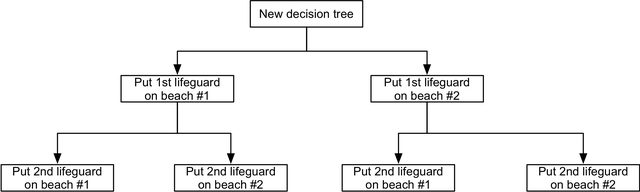
\includegraphics[scale=2]{decision_tree.png}}
    \label{decision_tree}
    \caption{Exemplo de Árvore de Decisão \cite{decision_tree}}
\end{figure}

A predição de uma classe é baseada essencialmente em percorrer o diagrama utilizando os valores dos atributos conhecidos
como entrada para as regras inferidas pelo modelo. A acurácia do modelo está, portanto, diretamente correlacionada à
inferência das regras e também ao tamanho que a árvore pode adotar, o que permite uma maior especificidade das regras
inferidas.

\subsection{Random Forest}

Modelos do tipo Random Forest realizam a agregação de diversas Árvores de Decisão (DT, do inglês \textit{decision tree}),
já explicadas na subseção \ref{decision_tree}, para composição de classificadores ou regressores. Para o problema
específico de classificação, a saída de uma Random Forest é a classe selecionada pela maioria das DTs. Já para
regressões, são retornadas as médias dos valores retornados por cada DT \cite{random_forest}.

O objetivo central na construção do modelo é diminuir a variância entre as saídas das DTs e ao mesmo tempo evitar
\textit{overfitting} - que ocorre quando o modelo é específico demais para o conjunto de treinamento e apresenta baixa
acurácia para conjuntos de teste. Para isso, o número de DTs utilizadas é configurável através de um hiperparâmetro, o
que permite realizar um ajuste que propicie a menor variância possível para análise.

\subsection{Gradient Boosting}

O método de Gradient Boosting preconiza a construção de um modelo preditivo forte a partir de modelos intermediários
fracos - ideia geral dos algoritmos de Boosting-, normalmente DTs. É similar, portanto, ao de Random Forest no que tange
a utilização de DTs como elementos de construção do modelo preditivo final. Diferem, entretanto, na forma como os
diferentes modelos intermediários (DTs) são agregados, já que no Gradient Boosting eles são sequencialmente adicionados,
enquanto em Random Forest são utilizados em paralelo.

O algoritmo de Gradient Boosting consiste em realizar o treinamento de um modelo fraco inicial e aplicar à ele próprio
uma função de correção a fim de melhorar a acurácia de um novo modelo a ser criado para o mesmo conjunto de dados. Nesse
caso, como o nome do método sugere, a função de correção é derivada do gradiente da função em cada etapa da interação,
conforme a seguinte equação:
\begin{equation}
    F_{m+1}(x) = F_m(x) + h_m(x)
\end{equation}

Onde $h_m(x)$ é a função de correção, que será o gradiente da função de avaliação utilizada para o problema. Além disso,
o método possui 3 hiperparâmetros: tamanho da árvore, taxa de aprendizado e subamostra. Os dois últimos servem,
respectivamente, para controlar a proporção em que a função de correção é adicionada e o particionamento da amostra
original durante a construção do modelo.

\subsection{SVM}

O método de Support Vector Machine (SVM) consiste na utilização das chamadas funções de núcleo para manipular o espaço
de características de um dado problema de forma indireta a fim de obter uma medida de similaridade entre diferentes
entradas do conjunto de dados. A partir da aplicação da função de núcleo, é construída então uma matriz de núcleo, que
contém uma representação do conjunto inicial com suas respectivas similaridades em relação a todos os outros registros.
Esse matriz é, posteriormente, utilizada para construção de um hiperplano que separa as diferentes classes alvo.

A fim de minimizar o erro de classificação produzido pelo método, o conceito de margem de separação é adotado no SVM, e
consiste em definir um limiar definido a partir do hiperplano para o qual o modelo é capaz de realizar classificações
corretas. Com isso, ao maximizarmos a margem de separação, chegamos ao modelo com a maior capacidade de classficar
corretamente os registros.

O modelo disponibiliza 2 hiperparâmetros, C e $\gamma$. O primeiro, C, é um parâmetro de regularização da SVM, e define a
margem utilizada pelo modelo para determinar o quanto de erro é aceitável. Isso permite controlar a troca entre a
fronteira de decisão e o termo de classificação errônea. Quando C estiver alto, o modelo classificará um número maior de
pontos, o que também pode ocasionar perda de acurácia e overfitting. Já o hiperparâmetro $\gamma$ define o quanto a
distância entre os pontos influencia o cálculo dos hiperplanos. Quanto maior for Gamma, mais influência possuem pontos
próximos e maior a probabilidade de overfitting. Por outro lado, quanto menor for Gamma, maior a influência de pontos
mais distantes e mais generalista o modelo.

\subsection{Redes Neurais}



\section{Resultados}
\label{resultados}

\subsection{Visualização e Caracterização dos dados}

\begin{figure}[htbp]
    \centerline{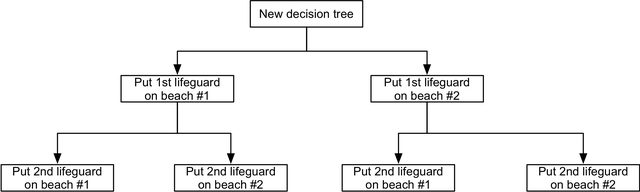
\includegraphics[scale=2]{decision_tree.png}}
    \label{decision_tree}
    \caption{Exemplo de Árvore de Decisão \cite{decision_tree}}
\end{figure}

Conforme apresentado na tabela \ref{attributes}, algumas colunas como \textit{agent} e \textit{company} possuem entradas
com valores nulos, cuja manutenção afetaria as análises efetuadas. Como a variável que define a empresa associada à
reserva é nula em 94\% das entradas, optou-se por removê-la. Aproveitou-se também para remover variáveis intuitivamente
irrelevantes para o modelo, como nome, e-mail e telefone. Após isso, foi possível remover todas as entradas contendo
valores nulos, já que representavam uma pequena parte do dataset utilizado ($\approx10\%$).

Como uma etapa de engenharia de atributos, optou-se por tratar algumas informações pouco relevantes para o modelo em sua
forma original. Para isso, um novo atributo de localização (\textit{guest\_location}) foi criado para substituir o
atributo de país, mapeando Portugal em "Local" e outros países em "Internacional", já que o número de reservas
provenientes de Portugal era inicialmente muito maior que as de outros países individualmente. Além disso, as variáveis
\textit{children} e \textit{babies} foram somadas em uma nova variável \textit{kids}. Por final, dois novos atributos
\textit{total\_guests} e \textit{total\_stays} foram criados a fim de representar, respectivamente, as somas de hóspedes
(adultos, crianças e bebês) e diárias (diárias em finais de semana e dias de semana).

Após as modificações citadas acima, realizou-se o procedimento de conversão de variáveis categóricas para variáveis
indicadoras. Por exemplo, a variável \textit{meal} foi dividida em 4 novas variáveis: \textit{meal\_FB}, \textit{meal\_HB},
\textit{meal\_SC} e \textit{meal\_Undefined}, que representam as diferentes possibilidades de refeições a serem escolhidas
pelos clientes.

\begin{itemize}
    \color{red}
        \item Visualização e Caracterização dos dados (distribuições, correlações, etc.)
        \item Descrição do procedimento de validação (validação cruzada)
        \item Resultados dos modelos lineares:
            \begin{enumerate}
                \item Regressão Linear / Regressão Logística
                \item Classificação Bayesiana (problemas de classificação)
            \end{enumerate}
        \item Resultados dos modelos não lineares
            \begin{enumerate}
                \item Árvores de decisão
                \item Random Forest (testar pelo menos 2 opções de hiperparâmetros)
                \item Gradient Boosting (testar pelo menos 2 opções de hiperparâmetros)
                \item SVM (testar pelo menos 2 opções de hiperparâmetros)
                \item Redes Neurais (testar pelo menos 3 topologias/hiperparâmetros)
            \end{enumerate}
        \item Discussão e comparação dos resultados
\end{itemize}

\section{Conclusões}

\begin{itemize}
    \color{red}
        \item Discussão sobre as características do problema
        \item Discussão dos resultados obtidos em função das características do problema
        \item Recomendação sobre o melhor modelo para a aplicação
        \item Trabalhos futuros (opcional)
\end{itemize}

\begin{thebibliography}{1}
    \bibitem{kaggle} \url{https://www.kaggle.com/mojtaba142/hotel-booking}. Acessado em 20/02/2022.
    \bibitem{colab} \url{https://colab.research.google.com/}.
    \bibitem{evsukoff} Evsukoff, A. Ensinando Máquinas, 2017.
    \bibitem{decision\_tree} M. Wagner, H. Principles of Operations Research, 1975.
    \bibitem{random_forest} \url{https://en.wikipedia.org/wiki/Random_forest}.
\end{thebibliography}

\end{document}
